We first briefly introduce the notion of loss functions and explain how the chain rule can be easily applied with expressions involving tensors and Jacobian tensors. A loss function $L:S\times S\to \RR^{\geq 0}$ serves to measure the error or cost incurred by a computational model, algorithm, or decision process when producing the output $\hat{y}\in S$ as a prediction of the ground truth $y\in S$. The goal of many learning and optimization algorithms is to minimize this loss. One approach is to use the Frobenius norm for the difference between the predicted output and the ground truth. To minimize the Frobenius norm when both the input and output are tensors, Jacobians can be used to compute the necessary gradients. Let $\At\in\RR^{d_1\times d_2\times d_3}$ be the ground truth and $\Tt\in\RR^{d_1\times d_2\times d_3}$ be the predicted output. Using Theorem~\ref{thm:gradients}, the gradient of the loss $L = \norm{\At-\Tt}_F^2$ can be written as:
    \begin{align*}
        \frac{\partial\norm{\At-\Tt}_F^2}{\partial\Tt} 
        &=
        \frac{\partial}{\partial\Tt}\left(\norm{\At}_F^2 + \norm{\Tt}_F^2 - 2\langle\At,\Tt\rangle\right)\\
        &= 
    \frac{\partial}{\partial\Tt}\left(\begin{tikzpicture}[baseline=\baseline]
    \tikzset{tensor/.style = {minimum size = 0.5cm,shape = circle,thick,draw=black,inner sep = 0pt}, edge/.style = {thick,line width=.4mm},every loop/.style={}}
    \def\y{0}
    \def\x{0}
    \node[tensor,fill=green!50!red!50!white] (St) at (\x,\y){\scalebox{0.85}{$\Tt$}};
    \node[tensor,fill=green!50!red!50!white] (Tt) at (\x+1,\y){\scalebox{0.85}{$\Tt$}};
    \draw[edge] (St) -- (Tt);
    \draw[edge] (St) to [out=45,in=135] (Tt);
    \draw[edge] (St) to [out=-45,in=-135] (Tt);
    \node[draw=none] () at (\x+0.5,\y+0.5) {\scalebox{0.7}{\dimcolor{$d_1$}}};
    \node[draw=none] () at (\x+0.5,\y+0.15) {\scalebox{0.7}{\dimcolor{$d_2$}}};
    \node[draw=none] () at (\x+0.5,\y-0.5) {\scalebox{0.7}{\dimcolor{$d_3$}}};
\end{tikzpicture}
-2
~
\begin{tikzpicture}[baseline=\baseline]
    \tikzset{tensor/.style = {minimum size = 0.5cm,shape = circle,thick,draw=black,inner sep = 0pt}, edge/.style = {thick,line width=.4mm},every loop/.style={}}
    \def\y{0}
    \def\x{0}
    \node[tensor,fill=blue!40!red!20!white] (St) at (\x,\y){\scalebox{0.85}{$\At$}};
    \node[tensor,fill=green!50!red!50!white] (Tt) at (\x+1,\y){\scalebox{0.85}{$\Tt$}};
    \draw[edge] (St) -- (Tt);
    \draw[edge] (St) to [out=45,in=135] (Tt);
    \draw[edge] (St) to [out=-45,in=-135] (Tt);
    \node[draw=none] () at (\x+0.5,\y+0.5) {\scalebox{0.7}{\dimcolor{$d_1$}}};
    \node[draw=none] () at (\x+0.5,\y+0.15) {\scalebox{0.7}{\dimcolor{$d_2$}}};
    \node[draw=none] () at (\x+0.5,\y-0.5) {\scalebox{0.7}{\dimcolor{$d_3$}}};
\end{tikzpicture}
\right)\\
&=
\left(\begin{tikzpicture}[baseline=\baseline]
    \tikzset{tensor/.style = {minimum size = 0.5cm,shape = circle,thick,draw=black,inner sep = 0pt}, edge/.style = {thick,line width=.4mm},every loop/.style={}}
    \def\y{0}
    \def\x{0}
    \node[tensor,fill=green!50!red!50!white] (Tt) at (\x,\y){\scalebox{0.85}{$\Tt$}};
    \draw[edge](Tt) -- (\x+0.85,\y)node[midway, above]{\edgelabel{$d_2$}};
    \draw[edge](Tt) -- (\x-0.85,\y)node[midway, above]{\edgelabel{$d_1$}};
    \draw[edge](Tt) -- (\x,\y-0.85)node[midway, left]{\edgelabel{$d_3$}};
    \end{tikzpicture}
+
\begin{tikzpicture}[baseline=\baseline]
    \tikzset{tensor/.style = {minimum size = 0.5cm,shape = circle,thick,draw=black,inner sep = 0pt}, edge/.style = {thick,line width=.4mm},every loop/.style={}}
    \def\y{0}
    \def\x{0}
    \node[tensor,fill=green!50!red!50!white] (Tt) at (\x,\y){\scalebox{0.85}{$\Tt$}};
    \draw[edge](Tt) -- (\x+0.85,\y)node[midway, above]{\edgelabel{$d_2$}};
    \draw[edge](Tt) -- (\x-0.85,\y)node[midway, above]{\edgelabel{$d_1$}};
    \draw[edge](Tt) -- (\x,\y-0.85)node[midway, left]{\edgelabel{$d_3$}};
    \end{tikzpicture}
-2~~
\begin{tikzpicture}[baseline=\baseline]
    \tikzset{tensor/.style = {minimum size = 0.5cm,shape = circle,thick,draw=black,inner sep = 0pt}, edge/.style = {thick,line width=.4mm},every loop/.style={}}
    \def\y{0}
    \def\x{0}
    \node[tensor,fill=blue!40!red!20!white] (Tt) at (\x,\y){\scalebox{0.85}{$\At$}};
    \draw[edge](Tt) -- (\x+0.85,\y)node[midway, above]{\edgelabel{$d_2$}};
    \draw[edge](Tt) -- (\x-0.85,\y)node[midway, above]{\edgelabel{$d_1$}};
    \draw[edge](Tt) -- (\x,\y-0.85)node[midway, left]{\edgelabel{$d_3$}};
    \end{tikzpicture}\right)\\
&=
2\left(\begin{tikzpicture}[baseline=\baseline]
    \tikzset{tensor/.style = {minimum size = 0.5cm,shape = circle,thick,draw=black,inner sep = 0pt}, edge/.style = {thick,line width=.4mm},every loop/.style={}}
    \def\y{0}
    \def\x{0}
    \node[tensor,fill=green!50!red!50!white] (Tt) at (\x,\y){\scalebox{0.85}{$\Tt$}};
    \draw[edge](Tt) -- (\x+0.85,\y)node[midway, above]{\edgelabel{$d_2$}};
    \draw[edge](Tt) -- (\x-0.85,\y)node[midway, above]{\edgelabel{$d_1$}};
    \draw[edge](Tt) -- (\x,\y-0.85)node[midway, left]{\edgelabel{$d_3$}};
    \end{tikzpicture}
-
\begin{tikzpicture}[baseline=\baseline]
    \tikzset{tensor/.style = {minimum size = 0.5cm,shape = circle,thick,draw=black,inner sep = 0pt}, edge/.style = {thick,line width=.4mm},every loop/.style={}}
    \def\y{0}
    \def\x{0}
    \node[tensor,fill=blue!40!red!20!white] (Tt) at (\x,\y){\scalebox{0.85}{$\At$}};
    \draw[edge](Tt) -- (\x+0.85,\y)node[midway, above]{\edgelabel{$d_2$}};
    \draw[edge](Tt) -- (\x-0.85,\y)node[midway, above]{\edgelabel{$d_1$}};
    \draw[edge](Tt) -- (\x,\y-0.85)node[midway, left]{\edgelabel{$d_3$}};
    \end{tikzpicture}\right).
\end{align*}
The chain rule can be easily extended to expressions involving tensor variables. Consider, for example, an arbitrary loss function $\mathcal{ L}: \mathbb{R}^{d_1\times \cdots \times d_N} \to \mathbb{R}$ that one wishes to minimize over the $N$-th order tensor inputs $\Tt$. Now suppose that the tensor input is parameterized as a tensor network where $\Gt \in \mathbb{R}^{m_1\times \cdots \times m_M}$ is an $M$-th order core tensor. To compute the Jacobian tensor of $\mathcal L$ with respect to $\Gt$, one can use the chain rule as follows: 
$$\frac{\partial  \mathcal L}{\partial\Gt} 
=
\frac{\partial \mathcal L}{\partial \Tt }\frac{\partial\Tt}{\partial\Gt}  $$
where $\frac{\partial  \mathcal L}{\partial\Gt}$ is of size $m_1\times\cdots \times m_M$, $\frac{\partial  \mathcal L}{\partial \Tt }$ is of size%
\footnote{One could say that,technically, $\frac{\partial  \mathcal L}{\partial\Gt}$ has shape $1\times m_1 \cdots \times m_M$  and $\frac{\partial  \mathcal L}{\partial \Tt }$ has shape $1\times d_1\times \cdots \times d_N$, but the first trivial mode of dimension $1$ is naturally omitted.}
$d_1\times \cdots \times d_N$, and $\frac{\partial\Tt}{\partial\Gt} $ is of size $d_1\times \cdots \times d_N \times m_1 \cdots \times m_M$. The product between $\frac{\partial  \mathcal L}{\partial \Tt }$ and $\frac{\partial\Tt}{\partial\Gt}  $ is implicitly understood as the contraction between the $M$ modes of $\frac{\partial  \mathcal L}{\partial \Tt }$ with the first $M$-modes  of $\frac{\partial\Tt}{\partial\Gt}  $.

We are now ready to conclude this chapter by presenting two applications of tensor network gradient computations. 
\begin{itemize}
\item\textbf{CP Decomposition with Gradient Descent} To find an approximate CP decomposition~(see Section~\ref{sec:cp-decomposition}) of a tensor $\Tt\in\RR^{d_1\times\cdots\times d_N}$, one can use gradient descent to minimize the loss $L = \norm{\Tt-\CP{\Gb_1,\cdots,\Gb_N}}^2_F$. Here $\CP{\Gb_1,\cdots,\Gb_N}$ denotes the CP decomposition where $\Gb_1,\cdots,\Gb_N$ are the factor matrices. To optimize w.r.t. the factor matrices, we can apply gradient descent to the loss function. For instance, in the case of $N=3$, to compute $\Gb_1$  we can apply the chain rule and write $\frac{\partial L}{\partial\Gb_1} = \frac{\partial L}{\partial\CP{\Gb_1,\Gb_2,\Gb_3}}\frac{\partial\CP{\Gb_1,\Gb_2,\Gb_3}}{\partial\Gb_1}$, where $\frac{\partial L}{\partial\CP{\Gb_1,\Gb_2,\Gb_3}}= 2(\Tt-\CP{\Gb_1,\Gb_2,\Gb_3})\in\RR^{d_1\times d_2\times d_3}$ and 
\begin{align*}
\frac{\partial\CP{\Gb_1,\Gb_2,\Gb_3}}{\partial\Gb_1}
=
\begin{tikzpicture}[baseline=\baseline]
    \tikzset{tensor/.style = {minimum size = 0.5cm,shape = circle,thick,draw=black,inner sep = 0pt}, edge/.style   = {thick,line width=.4mm},every loop/.style={}}
    \def\y{0}
    \def\x{0}
 \node[tensor,fill=blue!50!white] (G2) at (\x+1,\y){$\Gb_2$};
   \node[tensor,fill=blue!20!white] (G3) at (\x+2,\y){$\Gb_3$};
    \draw  node[fill = black,circle,inner sep=0pt,minimum size=4pt] (m) at (\x+1,\y+1) {};
    \draw[edge] (m) -- (\x,\y+0.1) node [midway,left] {\edgelabel{$R$}};
    \draw[edge] (G2) -- (m)node [midway,left] {\edgelabel{$R$}};
    \draw[edge] (G3) -- (m)node [midway,right] {\edgelabel{$R$}};
    \draw[edge](\x,\y-0.1) -- (\x,\y-0.7) node [midway,right] {\edgelabel{$d_1$}};
    \draw[edge](G2) -- (\x+1,\y-0.7)node [midway,left] {\edgelabel{$d_2$}};
    \draw[edge](G3) -- (\x+2,\y-0.7) node [midway,left] {\edgelabel{$d_3$}};
\end{tikzpicture}\in\RR^{d_1\times d_2\times d_3\times R}.
\end{align*}
Looking at the resulting TN, one can see that it can be expressed using matricizations and the Khatri-Rao product:
\begin{align*}
  \frac{\partial L}{\partial\Gb_1} 
&=
\frac{\partial L}{\partial\CP{\Gb_1,\Gb_2,\Gb_3}}\frac{\partial\CP{\Gb_1,\Gb_2,\Gb_3}}{\partial\Gb_1}\\
&=
\begin{tikzpicture}[baseline=-0.5ex]
    \tikzset{tensor1/.style = {minimum width = 3cm,minimum height = 0.6cm,shape = rounded rectangle,thick,draw=black,inner sep = 0pt}, edge/.style = {thick,line width=.4mm},every loop/.style={}}
     \tikzset{tensor2/.style = {minimum size = 0.5cm,shape = circle,thick,draw=black,inner sep = 0pt}, edge/.style   = {thick,line width=.4mm},every loop/.style={}}
    \def\y{1}
    \def\x{0}
    \node[tensor1,fill=blue!45!red!20!white] (Tt) at (\x,\y){$2(\Tt-\CP{\Gb_1,\Gb_2,\Gb_3})$};
    \node[tensor2,fill=blue!50!white] (G2) at (\x,\y-1){$\Gb_2$};
   \node[tensor2,fill=blue!20!white] (G3) at (\x+1,\y-1){$\Gb_3$};
    \draw  node[fill = black,circle,inner sep=0pt,minimum size=4pt] (m) at (\x+0.5,\y-1.85) {};
    \draw[edge](G2)--(m)node [midway,left] {\edgelabel{$R$}};
    \draw[edge](G3)--(m)node [midway,right] {\edgelabel{$R$}};    \draw[edge](Tt)--(G2)node [midway,left] {\edgelabel{$d_2$}};
    \draw[edge](\x+1,\y-0.3)--(G3)node [midway,left] {\edgelabel{$d_3$}};
    \draw[edge](m)--(\x+0.5,\y-2.25)node [midway,left] {\edgelabel{$R$}};
    \draw[edge](\x-0.75,\y-0.3) -- (\x-0.75,\y-2.25)node [midway,left] {\edgelabel{$d_1$}};
\end{tikzpicture}\\
&=\begin{tikzpicture}[baseline=-0.5ex]
    \tikzset{tensor/.style = {minimum width = 3cm,minimum height = 0.6cm,shape = rounded rectangle,thick,draw=black,inner sep = 0pt}, edge/.style = {thick,line width=.4mm},every loop/.style={}}
    \def\y{1}
    \def\x{0}
    \node[tensor,fill=blue!45!red!20!white] (Tt) at (\x,\y){$2(\Tt-\CP{\Gb_1,\Gb_2,\Gb_3})$};
    \node[tensor,fill=blue!25!red!45!white] (Gt) at (\x+1,\y-1){$\Gb_2\krao\Gb_3$};
    \draw[edge](\x+0.5,\y-0.3) -- (\x+0.5,\y-0.7);
    \draw[edge](\x+0.6,\y-0.3) -- (\x+0.6,\y-0.7)node [midway,right] {\edgelabel{$d_2d_3$}};
    \draw[edge](\x-0.75,\y-0.3) -- (\x-0.75,\y-2)node [midway,left] {\edgelabel{$d_1$}};
    \draw[edge](\x+0.85,\y-1.3) -- (\x+0.85,\y-2)node [midway,left] {\edgelabel{$R$}};
\end{tikzpicture}\\
&=
2(\Tt-\CP{\Gb_1,\Gb_2,\Gb_3})_{(1)}(\Gb_2\krao\Gb_3)
\in\RR^{d_1\times R}.
\end{align*}
 \item\textbf{Machine Learning} To compress neural networks, the dense weight matrices of fully connected layers can be parameterized using tensor factorizations to reduce memory usage~\citep{novikov2015tensorizing}. Let $\Wb\in\RR^{P\times D}$ be a weight matrix and $\xb\in\RR^{D}$ the input vector of a neural network layer. The output $\yb\in\RR^{P}$ is obtained by contracting the weight matrix $\Wb$ with the input vector $\xb$. 
    Suppose $P = \Pi_{i=1}^N{p_i}$ and $D =\Pi_{i=1}^Nd_i$. Then by reshaping $\Wb$ and $\xb$ in tensors we have
\begin{align*}
    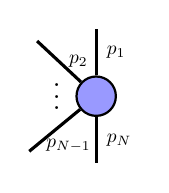
\begin{tikzpicture}[baseline=-0.1ex]
    \tikzset{tensor/.style = {minimum size = 0.5cm,shape = circle,thick,draw=black,inner sep = 0pt}, edge/.style = {thick,line width=.4mm},every loop/.style={}}
    \def\x{6}
    \def\y{0}
    \node[tensor,fill=blue!40!white] (y) at (\x,\y) {$\Yt$};
    \draw[edge](y)--(\x,\y+0.85)node [midway,right] {\scalebox{0.7}{\dimcolor{$p_1$}}};
    \draw[edge](y)--(\x-0.75,\y+0.7)node [midway,right=-0.01cm] {\scalebox{0.7}{\dimcolor{$p_2$}}};
    \draw[edge](y)--(\x-0.85,\y-0.7)node [very near end,right] {\scalebox{0.7}{\dimcolor{$p_{N-1}$}}};
    \draw[edge](y)--(\x,\y-0.85)node [midway,right] {\scalebox{0.7}{\dimcolor{$p_N$}}};
    \node[draw=none] at (\x-0.5,\y+0.1){$\vdots$};
    \end{tikzpicture}
=\sum_{d_1,\cdots,d_N}\Wt_{p_1,\cdots, p_N,d_1,\cdots, d_N}\Xt_{d_1,\cdots, d_N} =
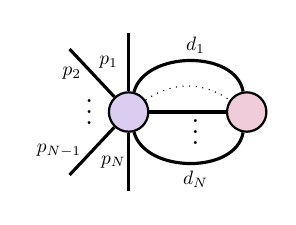
\begin{tikzpicture}[baseline=-0.1ex]
    \tikzset{tensor/.style = {minimum size = 0.5cm,shape = circle,thick,draw=black,inner sep = 0pt}, edge/.style = {thick,line width=.4mm},every loop/.style={}}
    \def\x{6}
    \def\y{0}
    \node[tensor,fill=red!30!blue!20!white] (w) at (\x,\y) {$\Wt$};
    \node[tensor,fill=blue!30!red!20!white] (x) at (\x+1.5,\y) {$\Xt$};
    \draw[edge](w)--(x);
    \draw[edge](w)--(\x,\y+1)node [midway,left] {\scalebox{0.7}{\dimcolor{$p_1$}}};
    \draw[edge](w)--(\x-0.75,\y+0.8)node [midway,left] {\scalebox{0.7}{\dimcolor{$p_2$}}};
    \draw[edge](w)--(\x-0.75,\y-0.8)node [midway,left] {\scalebox{0.7}{\dimcolor{$p_{N-1}$}}};
    \draw[edge](w)--(\x,\y-1)node [midway,left=-0.1cm] {\scalebox{0.7}{\dimcolor{$p_N$}}};
    \node[draw=none] at (\x-0.5,\y+0.1){$\vdots$};
   \draw[edge] (w) to [out=-75,in=-100] (x);
    \draw[edge] (w) to [out=75,in=100] (x);
    \draw[dotted] (w) to [out=35,in=145] (x);
    \node[draw=none] at (\x+0.85,\y-0.15){$\vdots$};
    \node[draw=none] () at (\x+0.85,\y+0.85) {\scalebox{0.7}{\dimcolor{$d_1$}}};
    (\x+1.2,\y-0.2){$\vdots$};
    \node[draw=none] () at (\x+0.85,\y-0.85) {\scalebox{0.7}{\dimcolor{$d_N$}}};
\end{tikzpicture}.
\end{align*}
For simplicity, we proceed with the case $N=4$. In~\citep{novikov2015tensorizing}, the authors propose to parameterize $\Wt$ in the MPO format~(see Section~\ref{sec:efficient-operations}). i.e., 
$\Wt = 
\begin{tikzpicture}[baseline=\baseline]
    \tikzset{tensor/.style = {minimum size = 0.5cm,shape = circle,thick,draw=black,inner sep = 0pt}, edge/.style   = {thick,line width=.4mm},every loop/.style={}}
    \def\y{0}
    \def\x{0}
  \node[tensor,fill=red!30!white] (G1) at (\x,\y){$\Gt_1$};
  \node[tensor,fill=red!50!white] (G2) at (\x+1,\y){\scalebox{0.85}{$\Gt_2$}};
  \node[tensor,fill=blue!30!white] (G3) at (\x+2,\y){$\Gt_3$};
  \node[tensor,fill=blue!50!white] (G4) at (\x+3,\y){$\Gt_4$};
    \draw[edge](G1) -- (\x,\y-0.85)node [midway,left] {\edgelabel{$d_1$}};
    \draw[edge](G2) -- (\x+1,\y-0.85)node [midway,left] {\edgelabel{$d_2$}};
     \draw[edge](G3) -- (\x+2,\y-0.85)node [midway,left] {\edgelabel{$d_3$}};
    \draw[edge](G4) -- (\x+3,\y-0.85)node [midway,left] {\edgelabel{$d_4$}};
    \draw[edge](G1) -- (G2) node [midway,above] {\edgelabel{$R_1$}};
    \draw[edge](G2) -- (G3) node [midway,above] {\edgelabel{$R_2$}};
    \draw[edge](G3) -- (G4) node [midway,above] {\edgelabel{$R_3$}};
    \draw[edge](G1) -- (\x,\y+0.85)node [midway,left] {\edgelabel{$p_1$}};
    \draw[edge](G2) -- (\x+1,\y+0.85)node [midway,left] {\edgelabel{$p_2$}};
    \draw[edge](G3) -- (\x+2,\y+0.85)node [midway,left] {\edgelabel{$p_3$}};
    \draw[edge](G4) -- (\x+3,\y+0.85)node [midway,left] {\edgelabel{$p_4$}};
\end{tikzpicture}.$
During the backpropagation step, since we aim to update the weight matrix, we need to optimize it with respect to all the core tensors. According to the chain rule, this gives: $\frac{\partial L}{\partial \Gt_i} = \frac{\partial L}{\partial \Yt}\frac{\partial\Yt}{\partial\Gt_i}$ for $i\in[4]$, where $L$ denotes the loss function. For instance, for $i=2$ we need to find the derivative of $\Yt$ with respect to $\Gt_2$. By applying Theorem~\ref{thm:gradients} we just need to remove $\Gt_2$ from the tensor network to obtain the result:
\begin{align*}
\frac{\partial\Yt}{\partial\Gt_2} 
&=
\frac{\partial\left(\begin{tikzpicture}[baseline=\baseline]
    \tikzset{tensor/.style = {minimum size = 0.5cm,shape = circle,thick,draw=black,inner sep = 0pt}, edge/.style   = {thick,line width=.4mm},every loop/.style={}}
    \def\y{0}
    \def\x{0}
  \node[tensor,fill=red!30!white] (G1) at (\x,\y){$\Gt_1$};
  \node[tensor,fill=red!50!white] (G2) at (\x+1,\y){\scalebox{0.85}{$\Gt_2$}};
  \node[tensor,fill=blue!30!white] (G3) at (\x+2,\y){$\Gt_3$};
  \node[tensor,fill=blue!50!white] (G4) at (\x+3,\y){$\Gt_4$};
  \node[tensor,fill=blue!30!red!20!white] (x) at (\x+1.5,\y-1.5) {$\Xt$};
    \draw[edge](G1) -- (\x,\y-0.85)node [midway,left] {\edgelabel{$d_1$}};
    \draw[edge](x)--(\x,\y-0.85);
    \draw[edge](G2) -- (\x+1,\y-0.85)node [midway,left] {\edgelabel{$d_2$}};
    \draw[edge](x)--(\x+1,\y-0.85);
     \draw[edge](G3) -- (\x+2,\y-0.85)node [midway,left] {\edgelabel{$d_3$}};
    \draw[edge](x)--(\x+2,\y-0.85);
    \draw[edge](G4) -- (\x+3,\y-0.85)node [midway,left] {\edgelabel{$d_4$}};
    \draw[edge](x)--(\x+3,\y-0.85);
    \draw[edge](G1) -- (G2) node [midway,above] {\edgelabel{$R_1$}};
    \draw[edge](G2) -- (G3) node [midway,above] {\edgelabel{$R_2$}};
    \draw[edge](G3) -- (G4) node [midway,above] {\edgelabel{$R_3$}};
    \draw[edge](G1) -- (\x,\y+0.85)node [midway,left] {\edgelabel{$p_1$}};
    \draw[edge](G2) -- (\x+1,\y+0.85)node [midway,left] {\edgelabel{$p_2$}};
    \draw[edge](G3) -- (\x+2,\y+0.85)node [midway,left] {\edgelabel{$p_3$}};
    \draw[edge](G4) -- (\x+3,\y+0.85)node [midway,left] {\edgelabel{$p_4$}};
\end{tikzpicture}\right)}{\partial\Gt_2}\\
&=
\begin{tikzpicture}[baseline=\baseline]
    \tikzset{tensor/.style = {minimum size = 0.5cm,shape = circle,thick,draw=black,inner sep = 0pt}, edge/.style   = {thick,line width=.4mm},every loop/.style={}}
    \def\y{-1}
    \def\x{0}
  \node[tensor,fill=red!30!white] (G1) at (\x,\y+1.5){$\Gt_1$};
    \node[tensor,fill=blue!30!white] (G3) at (\x+2,\y+1.5){$\Gt_3$};
  \node[tensor,fill=blue!50!white] (G4) at (\x+3,\y+1.5){$\Gt_4$};
  \node[tensor,fill=blue!30!red!20!white] (x) at (\x+1.5,\y) {$\Xt$};
    \draw[edge](G1) -- (\x,\y+0.85)node [midway,left] {\edgelabel{$d_1$}};
    \draw[edge](x)--(\x,\y+0.85);
    \draw[edge](\x+1,\y+1.35) -- (\x+1,\y+0.85)node [midway,left] {\edgelabel{$d_2$}};
    \draw[edge](x)--(\x+1,\y+0.85);
     \draw[edge](G3) -- (\x+2,\y+0.85)node [midway,left] {\edgelabel{$d_3$}};
    \draw[edge](x)--(\x+2,\y+0.85);
    \draw[edge](G4) -- (\x+3,\y+0.85)node [midway,left] {\edgelabel{$d_4$}};
    \draw[edge](x)--(\x+3,\y+0.85);
    \draw[edge](G3) -- (G4) node [midway,above] {\edgelabel{$R_3$}};
    \draw[edge](G1) -- (\x,\y+2.35)node [midway,left] {\edgelabel{$p_1$}};
    \draw[edge](G3) -- (\x+2,\y+2.35)node [midway,left] {\edgelabel{$p_3$}};
    \draw[edge](G4) -- (\x+3,\y+2.35)node [midway,left] {\edgelabel{$p_4$}};
    \draw[edge](G1)--(\x+0.85,\y+1.5) node [midway,above] {\edgelabel{$R_1$}};
    \draw[edge](G3)--(\x+1.25,\y+1.5) node [midway,above] {\edgelabel{$R_2$}};
    \draw[edge](\x+1,\y+1.6)--(\x+1,\y+2.35) node [midway,left] {\edgelabel{$p_2$}};
\end{tikzpicture}\in\RR^{p_1\times R_1\times p_2\times R_2\times p_3\times p_4\times d_2}.
\end{align*}
The gradient of the loss is thus given by
\begin{align*}
    \frac{\partial L}{\partial\Gt_2} = \frac{\partial L}{\partial\Yt}\frac{\partial \Yt}{\partial\Gt_2}
    =
    \begin{tikzpicture}[baseline=\baseline]
    \tikzset{tensor/.style = {minimum size = 0.5cm,shape = circle,thick,draw=black,inner sep = 0pt}, edge/.style   = {thick,line width=.4mm},every loop/.style={}}
    \def\y{-1.5}
    \def\x{0}
    \node[tensor,fill=green!30!white] (L) at (\x+1.5,\y+3.25){$\frac{\partial L}{\partial\Yt}$};
  \node[tensor,fill=red!30!white] (G1) at (\x,\y+1.5){$\Gt_1$};
    \node[tensor,fill=blue!30!white] (G3) at (\x+2,\y+1.5){$\Gt_3$};
  \node[tensor,fill=blue!50!white] (G4) at (\x+3,\y+1.5){$\Gt_4$};
  \node[tensor,fill=blue!30!red!20!white] (x) at (\x+1.5,\y) {$\Xt$};
    \draw[edge](G1) -- (\x,\y+0.85)node [midway,left] {\edgelabel{$d_1$}};
    \draw[edge](x)--(\x,\y+0.85);
    \draw[edge](\x+1,\y+1.35) -- (\x+1,\y+0.85)node [midway,left] {\edgelabel{$d_2$}};
    \draw[edge](x)--(\x+1,\y+0.85);
     \draw[edge](G3) -- (\x+2,\y+0.85)node [midway,left] {\edgelabel{$d_3$}};
    \draw[edge](x)--(\x+2,\y+0.85);
    \draw[edge](G4) -- (\x+3,\y+0.85)node [midway,left] {\edgelabel{$d_4$}};
    \draw[edge](x)--(\x+3,\y+0.85);
    \draw[edge](G3) -- (G4) node [midway,above] {\edgelabel{$R_3$}};
    \draw[edge](G1) -- (\x,\y+2.35)node [midway,left] {\edgelabel{$p_1$}};
    \draw[edge](L)--(\x,\y+2.35);
    \draw[edge](G3) -- (\x+2,\y+2.35)node [midway,left] {\edgelabel{$p_3$}};
    \draw[edge](L)--(\x+2,\y+2.35);
    \draw[edge](G4) -- (\x+3,\y+2.35)node [midway,left] {\edgelabel{$p_4$}};
    \draw[edge](L)--(\x+3,\y+2.35);
    \draw[edge](G1)--(\x+0.85,\y+1.5) node [midway,above] {\edgelabel{$R_1$}};
    \draw[edge](G3)--(\x+1.25,\y+1.5) node [midway,above] {\edgelabel{$R_2$}};
    \draw[edge](\x+1,\y+1.6)--(\x+1,\y+2.35) 
    node [midway,left] {\edgelabel{$p_2$}};
    \draw[edge](L)--(\x+1,\y+2.35);
\end{tikzpicture}\in\RR^{R_1\times p_2\times R_2\times d_2}.
\end{align*}

\end{itemize}






